\documentclass[ALICE,manyauthors]{cernphprep}

\usepackage[comma,square,numbers,sort&compress]{natbib}
\usepackage{hyperref}
\usepackage{lineno}
%\usepackage{subcaption}
\usepackage{subfigure}
\usepackage[section]{placeins}
\usepackage {multicol}% Multi column in the table
\usepackage {multirow}% Multi row in the table
\usepackage {units}

\linenumbers

% $Id: commands.tex 934 2013-06-19 20:56:45Z mfloris $

\newcommand{\mrm}[1]{\mathrm{#1}}
\newcommand{\mrmo}[1]{\mathrm{\overline{#1}}}
\newcommand{\bsb}[1]{\boldsymbol{#1}}
\newcommand{\circit}{\item[$\circ$]}

\newcommand{\ITS}          {\rm{ITS}}
\newcommand{\TOF}          {\rm{TOF}}
\newcommand{\ZDC}          {\rm{ZDC}}
\newcommand{\ZDCs}         {\rm{ZDCs}}
\newcommand{\ZNA}          {\rm{ZNA}}
\newcommand{\ZNC}          {\rm{ZNC}}
\newcommand{\SPD}          {\rm{SPD}}
\newcommand{\SDD}          {\rm{SDD}}
\newcommand{\SSD}          {\rm{SSD}}
\newcommand{\TPC}          {\rm{TPC}}
\newcommand{\VZERO}        {\rm{VZERO}}
\newcommand{\VZEROA}       {\rm{VZERO-A}}
\newcommand{\VZEROC}       {\rm{VZERO-C}}
\newcommand{\pip}          {$\pi^{+}$}
\newcommand{\pim}          {$\pi^{-}$}
\newcommand{\kap}          {K$^{+}$}
\newcommand{\kam}          {K$^{-}$}
\newcommand{\pbar}         {$\rm\overline{p}$}
\newcommand{\kzero}        {\ensuremath{{\rm K}^{0}_{S}}}
\newcommand{\kstar}        {\ensuremath{{\rm K}^{*}}}
\newcommand{\He}           {\ensuremath{^{3}{\rm He}}}
\newcommand{\LH}           {\ensuremath{^{3}_{\Lambda}{\rm H}}}
\newcommand{\vzero}        {\ensuremath{{\rm V}^0}}
\newcommand{\lmb}          {\ensuremath{\Lambda}}
\newcommand{\almb}         {\ensuremath{\bar{\Lambda}}}
\newcommand{\allpart}      {$\pi^{\pm}$, K$^{\pm}$, \kzero, p(\pbar) and \lmb(\almb)}
\newcommand{\allpi}        {$\pi^{\pm}$}
\newcommand{\allk}         {K$^{\pm}$}
\newcommand{\allp}         {p(\pbar)}
\newcommand{\alllmb}       {\lmb(\almb)}
\newcommand{\degree}       {$^{\rm o}$}
\newcommand{\dg}           {\mbox{$^\circ$}}
\newcommand{\dedx}         {\ensuremath{\mathrm{d}E/\mathrm{d}x}}
\newcommand{\dndy}         {d$N$/d$y$}
\newcommand {\ee}            {\mbox{e$^+$e$^-$}}
\newcommand{\pp}           {pp}
\newcommand{\ppbar}        {\mbox{$\mathrm {p\overline{p}}$}}
\newcommand{\PbPb}         {\mbox{Pb--Pb}}
\newcommand{\pPb}          {\mbox{p--Pb}}
\newcommand{\AuAu}         {\mbox{Au--Au}}
\newcommand{\pseudorap}    {\mbox{$\left | \eta \right | $}}
\newcommand{\dNdeta}       {\ensuremath{\mathrm{d}N_\mathrm{ch}/\mathrm{d}\eta}}
\newcommand{\dNdy}         {\ensuremath{\mathrm{d}N/\mathrm{d}y}}
\newcommand{\dNdptdy}      {\ensuremath{\mathrm{d}N/{\rm d}\pt\mathrm{d}y}}
\newcommand{\dNdyst}       {\ensuremath{\sqrt{\frac{dN_\pi/dy}{s_T}}}}
\newcommand{\dNdetatr}     {\mathrm{d}N_\mathrm{tracklets}/\mathrm{d}\eta}
\newcommand{\dNdetar}[1]   {\mathrm{d}N_\mathrm{ch}/\mathrm{d}\eta\left.\right|_{|\eta|<#1}}
\newcommand{\lum}          {\, \mbox{${\rm cm}^{-2} {\rm s}^{-1}$}}
\newcommand{\barn}         {\, \mbox{${\rm barn}$}}
\newcommand{\m}            {\, \mbox{${\rm m}$}}
\newcommand{\ncls}         {\ensuremath{N_{cls}}}
\newcommand{\nsigma}       {\ensuremath{n\sigma}}
\newcommand{\dcaxy}        {\ensuremath{{\rm DCA}_{xy}}}
\newcommand{\dcaz}         {\ensuremath{{\rm DCA}_{z}}}
\newcommand{\EcrossB}      {E$\times$B}%{\ensuremath{{\rm E}\times{\rm B}}}
\newcommand{\bb}           {Bethe-Bloch}
\newcommand{\s}            {\ensuremath{\sqrt{s}}}
\newcommand{\pt}           {\ensuremath{p_\mathrm{T}}}
\newcommand{\pT}           {\ensuremath{p_{\rm T}}}
\newcommand{\hlab}         {\ensuremath{\eta_{\rm lab}}}
\newcommand{\ynn}         {\ensuremath{y_{\rm NN}}}
\newcommand{\ycms}         {\ensuremath{y_{\rm CMS}}}
\newcommand{\ylab}         {\ensuremath{y_{\rm lab}}}
\newcommand{\ppi}          {\ensuremath{{\rm p}/\pi}}
\newcommand{\kpi}          {\ensuremath{{\rm K}/\pi}}
\newcommand{\lpi}          {\ensuremath{{\rm \Lambda}/\pi}}
%\newcommand{\ppi}          {\ensuremath{(\pi^+ + \pi^-)/({\rm K}^+ + {\rm K}^-)}}
%\newcommand{\kpi}          {\ensuremath{({\rm p} + {\rm \bar p})/({\rm K}^+ + {\rm K}^-)}}
\newcommand{\mt}           {\ensuremath{m_{\rm T}}}
\newcommand{\snn}          {\ensuremath{\sqrt{s_{\rm NN}}}}
\newcommand{\snnbf}        {\ensuremath{\mathbf{{\sqrt{s_{\mathbf NN}}}}}}
\newcommand{\sonly}        {\ensuremath{\sqrt{s}}}
\newcommand{\Npart}        {\ensuremath{N_\mathrm{part}}}
\newcommand{\avNpart}      {\ensuremath{\langle N_\mathrm{part} \rangle}}
\newcommand{\avNpartdata}  {\ensuremath{\langle N_\mathrm{part}^{\rm data} \rangle}}
\newcommand{\Ncoll}        {\ensuremath{N_\mathrm{coll}}}
\newcommand{\Dnpart}       {\ensuremath{D\left(\Npart\right)}}
\newcommand{\DnpartExp}    {\ensuremath{D_{\rm exp}\left(\Npart\right)}}
\newcommand{\dNdetapt}     {\ensuremath{\dNdeta\,/\left(0.5\Npart\right)}}
\newcommand{\dNdetaptr}[1] {\ensuremath{\dNdetar{#1}\,/\left(0.5\Npart\right)}}
\newcommand{\dNdetape}     {\left(\ensuremath{\dNdeta\right)/\left(\avNpart/2\right)}}
\newcommand{\dNdetaper}[1] {\ensuremath{\dNdetar{#1}\,/\left(\avNpart/2\right)}}
\newcommand{\dndydpt}      {\ensuremath{{\rm d}^2N/({\rm d}y {\rm d}p_{\rm t})}}
\newcommand{\abs}[1]       {\ensuremath{\left|#1\right|}}
\newcommand{\signn}        {\ensuremath{\sigma^{\rm inel.}_{\rm NN}}}
\newcommand{\vz}           {\ensuremath{V_{z}}}
\newcommand{\Tfo}          {\ensuremath{{T}_{\rm kin}}}
\newcommand{\Tch}          {\ensuremath{{T}_{\rm ch}}}
\newcommand{\bT}           {\ensuremath{\beta_{\rm T}}}
\newcommand{\avbT}         {\ensuremath{\left< \beta_{\rm T}\right>}}
\newcommand{\avpT}         {\ensuremath{\left< \pt \right>}}
\newcommand{\muB}          {\ensuremath{\mu_{B}}}
\newcommand{\stat}         {({\it stat.})}
\newcommand{\syst}         {({\it sys.})}
\newcommand{\Fig}[1]       {Fig.~\ref{#1}}
\newcommand{\Figure}[1]    {Figure~\ref{#1}}
%\newcommand{\Ref}[1]       {Ref.~\cite{#1}}
%\newcommand{\green}[1]     {\textcolor{green}{#1}}
%\newcommand{\blue}[1]      {\textcolor{blue}{#1}}
%\newcommand{\red}[1]       {\textcolor{red}{#1}}
%\newcommand{\white}[1]     {\textcolor{white}{#1}}
\newcommand{\gevc}         {\ensuremath{{\rm GeV}/c}}
\newcommand{\mevc}         {\ensuremath{{\rm MeV}/c}}
\newcommand{\gs}           {\ensuremath{\gamma_{s}}}
\newcommand{\gq}           {\ensuremath{\gamma_{q}}}
\newcommand{\gc}           {\ensuremath{\gamma_{c}}}
\newcommand{\chindf}       {\ensuremath{\chi^{2}/{\rm NDF}}}
\newcommand{\avg}[1]       {\ensuremath{\left\langle#1\right\rangle}}
\newcommand{\etalab}       {\ensuremath{\eta_{{\rm lab}}}}
\newcommand {\gammas}			{\ensuremath{\gamma_{\mathrm{s}}}}

\newcommand{\DNDETAINEL}{5.31~$\pm$~0.18\xspace}
\newcommand{\DNDETAINELGTZERO}{6.46~$\pm$~0.19\xspace}
\newcommand{\DNDETAINELGTZEROONE}{6.61~$\pm$~0.20\xspace}

\newcommand{\inelgtzero}{INEL$>$0\xspace}
\newcommand{\average}[1]{\ensuremath{\langle #1 \rangle}\xspace}
\newcommand{\mpt}        {\ensuremath{\langle\pt\rangle}\xspace}
\newcommand{\nch}        {\ensuremath{N_\mathrm{ch}}\xspace}
\newcommand{\mnch}      {\ensuremath{\langle\nch\rangle}\xspace}
\newcommand{\nchacc}        {\ensuremath{N_\mathrm{ch}^\mathrm{acc}}\xspace}
\newcommand{\mnchacc}      {\ensuremath{\langle\nchacc\rangle}\xspace}
\newcommand{\inelg}     {\ensuremath{\mathrm{INEL}_{>0}}}



\newcommand{\dndeta}{\ensuremath{{\rm d}N_{\rm ch}/{\rm d}\eta}\xspace}
\newcommand{\dndpt}{\ensuremath{{\rm d}N_{\rm ch}/{\rm d}\pt}\xspace}
\newcommand{\etaless}[1]{\ensuremath{\left|\eta\right| < #1}\xspace}
\newcommand{\dndetaless}[1]{\ensuremath{{\rm d}N_{\rm ch}/{\rm d}\eta|_{\etaless{#1}}}\xspace}
\newcommand{\avdndeta}{\ensuremath{\langle \dndeta \rangle}}
\newcommand{\zvtx}{\ensuremath{z_\mathrm{vtx}}}
\newcommand{\pythiae}{\ensuremath{\mathrm{PYTHIA}\,8}}
%\newcommand{\pythiam}{\ensuremath{\mathrm{PYTHIA}\,8\,\mathrm{Monash}\,2013}}
\newcommand{\pythiam}{\ensuremath{\mathrm{PYTHIA}\,8\,\mathrm{Tune\,4C}}}
\newcommand{\pythiashoving}{{\ensuremath{\mathrm{PYTHIA}\,8~\mathrm{String}~}}\ensuremath{\mathrm{Shoving}}}
\newcommand{\epos}{{\ensuremath{\mathrm{EPOS}\,~\mathrm{LHC}}}}
%\newcommand{\pythiashoving}{\ensuremath{\mathrm{PYTHIA}\,8~\mathrm{String}~}\linenomath{-}\ensuremath{\mathrm{Shoving}}}
\newcommand{\pttrig}{\ensuremath{p_\mathrm{T,\,trig}}}
\newcommand{\ptassoc}{\ensuremath{p_\mathrm{T,\,assoc}}}
\newcommand{\ptjet}{\ensuremath{p_\mathrm{T,\,jet}^\mathrm{ch}}}
\newcommand{\ptlead}{\ensuremath{p_\mathrm{T,\,LP}}}
\newcommand{\pttrigassoc}{\ensuremath{p_\mathrm{T,\,trig\,(assoc)}}}









\renewcommand{\labelitemi} {$-$}
%==========================================================%
%%% inline warnings for internal discussion
%\newcommand{\warn}[1]      {\textbf{\textcolor{red}{[#1]}}}
\newcommand{\warn}[1]      {{\small\textbf{\textcolor{red}{(!\footnote{\textbf{(!)}~#1})}}}}
\newcommand{\warnin}[1]         {\textit{\textcolor{red}{(#1)}}}
%\newcommand{\warn}[1]      {#1}
%\newcommand{\warn}[1]      {{\small\textbf{(!\footnote{\textbf{(!)}~#1})}}\marginpar{\textbf{---}}}
\newcommand{\todo}[1]      {\textbf{\textcolor{red}{[TODO: #1]}}}
%%% fake numbers
\newcommand{\fake}[1]      {\textbf{\textcolor{red}{#1}}}
%\newcommand{\fake}[1]      {#1}
\newcommand{\final}[1]     {\textbf{\textcolor{blue}{#1}}}
\newcommand{\prelim}[1]    {\textbf{\textcolor{magenta}{#1}}}
\renewcommand{\mod}[1]       {\textbf{\textcolor{red}{#1}}}

\begin{document}

%%%%%%%%%%%%%%%  Title page %%%%%%%%%%%%%%%%%%%%%%%%
\begin{titlepage}

\PHyear{}
\PHnumber{2019-xxx}      % required, will be obtained from PH
%\PHdate{Day Month}  % required, will be obtained from PH
\PHdate{\today}
%

%%% Put your own title + short title here:
\title{Long-range correlations  in high-multiplicity  proton--proton collisions  at \s~=~\unit[13]{TeV} with ALICE at the LHC}
\ShortTitle{Long-range correlations in pp collisions}   % appears on right page headers

%%% Do not change the next lines
%\Collaboration{ALICE Collaboration\thanks{See Appendix~\ref{app:collab} for the list of collaboration members}}
\ShortAuthor{ALICE Collaboration} % appears on left page headers, do not change

\begin{abstract}

The observed azimuthal modulations of long-range correlations in pseudorapidity in small systems like pp or p-Pb collisions show strikingly similar features to those seen in heavy ion collisions. Many theoretical approaches to interpreting this effect have been developed. However, it is still unclear whether these long-range correlations are due to final or initial state effects. To further investigate these effects, we studied long-range correlations as a function of transverse momentum in very high multiplicity pp collisions at $\sqrt{s} =13$ TeV, collected with the high multiplicity event trigger during 2016 and 2017 with ALICE. In this talk, we present the near-side per-trigger yield at large pseudorapidity separation (ridge yield) as a function of transverse momentum in pp collisions at $\sqrt{s} =13$ TeV. The results are compared to previous measurements from CMS and ATLAS experiments. In addition, we present the ridge yield in events where harder fragmentation processes are present, to explore possible physical origins of long-range correlations.

\end{abstract}
\end{titlepage}
\setcounter{page}{2}



\section{Introduction}

%Studies of particle correlations in high-energy hadronhadron collisions provide valuable information on the underlying quantum chromodynamics processes leading to particle production. Measurements of two-particle angular correlations are typically performed in terms of twodimensional Δη-Δϕ correlation functions, where η is the pseudorapidity and ϕ is the azimuthal angle. Of particular interest in studies of possible novel partonic collective effects is the long-range (e.g., jΔηj > 2.0) structure of twoparticle correlation functions, in which the effects of known sources such as resonance decays and fragmentation of high-momentum partons are known to be small. In most Monte Carlo (MC) event generators for proton-proton (pp) collisions, the typical sources of such long-range correlations are momentum conservation and away-side (Δϕ ≈ π) jet correlations. Measurements in high-energy nucleusnucleus collisions have shown a long-range structure in the two-particle angular correlations functions, which has been attributed to the presence of the hot and dense matter formed [1]. Several novel features were observed in azimuthal correlations over large Δη for intermediate particle transverse momenta, pT ≈ 1–5 GeV=c [2,3]. These correlations are thought to arise from the response of a hydrodynamically expanding partonic medium to fluctuations of the initial collision geometry [4–9]. Measurements in pp collisions at a center-of-mass energy of ffiffi s p ¼ 7 TeV have also revealed the presence of long-range, near-side (Δϕ ≈ 0) correlations in events with very large final-state particle multiplicity [10]. Similar phenomena have also been observed in high-multiplicity proton-lead (pPb) collisions [11–13], where they have been studied extensively [14–21]. A wide range of models have been suggested to explain the emergence of these correlations in pp [22] and pPb [23–27] collisions. While models based on a hydrodynamic approach can describe many aspects of the observed correlations [23,24], it has been proposed that initial-state correlations of gluon fields could also lead to similar effects [25–27].

%Two-particle correlations are a powerful tool to explore the mechanism of particle production in collisions of hadrons and nu-clei at high energy. Such studies involve measuring the distribu-tions of relative anglesφandηbetween pairs of particles: a“trigger” particle in a certain transverse momentumpT,trigintervaland an “associated” particle in apT,associnterval, whereφandηare the differences in azimuthal angleφand pseudorapidityηbetween the two particles.In proton–proton (pp) collisions, the correlation at (φ≈0,η≈0) forpT,trig>2GeV/cis dominated by the “near-side” jetpeak, where trigger and associated particles originate from a frag-menting parton, and atφ≈πby the recoil or “away-side” jet[1].The away-side structure is elongated alongηdue to the longitu-dinal momentum distribution of partons in the colliding protons.In nucleus–nucleus collisions, the jet-related correlations are mod-ified and additional structures emerge, which persist over a longrange inηon the near side and on the away side[2–14].Theshape of these distributions when decomposed into a Fourier se-ries defined byvncoefficients[15]is found to be dominated bycontributions from terms withn=2 andn=3 [6,7,9–14].Thevncoefficients are sensitive to the geometry of the initial stateof the colliding nuclei[16,17]and can be related to the transport properties of the strongly-interacting de-confined matter via hy-drodynamic models[18–20].Recently, measurements in pp collisions at a centre-of-massenergy√s=7TeV[21]and in proton–lead (p–Pb) collisions ata nucleon–nucleon centre-of-mass energy√sNN=5.02 TeV[22]have revealed long-range (2<|η|<4) near-side (φ≈0) cor-relations in events with significantly higher-than-average particlemultiplicity. Various mechanisms have been proposed to explainthe origin of these ridge-like correlations in high-multiplicity ppand p–Pb events. These mechanisms include colour connectionsforming along the longitudinal direction[23–26], jet-medium[27]and multi-parton induced[28,29]interactions, and collective ef-fects arising in the high-density system possibly formed in thesecollisions[30–35].Results from two-particle correlations in√sNN=0.2TeVd–Aucollisions[36,37]show a strong suppression of the away-side yieldat forward rapidity in central collisions. This modification has beeninterpreted in the framework of “Colour Glass Condensate” mod-els [38]as a saturation effect caused by nonlinear gluon inter-actions in the high-density regime at small longitudinal partonmomentum fractionx. Similar effects may arise at midrapidity inp–Pb collisions at√sNN=5.02 TeV, where the parton distributionsare probed down tox<10−3, which is comparable to the relevantrange ofxat forward rapidity (y∼3) at√sNN=0.2TeV.This Letter presents results extracted from two-particle cor-relation measurements in p–Pb collisions at√sNN=5.02 TeV,recorded with the ALICE detector[39]at the Large Hadron Col-lider (LHC). The correlations are measured over two units of pseudorapidity and full azimuthal angle as a function of charged-particle multiplicity, and expressed as associated yield per triggerparticle. Sections2 and 3describe the experimental setup, andthe event and track selection, respectively. Details on the defini-tion of the correlation and the per-trigger-particle associated yieldare given in Section4. The results of the analysis are discussed inSection5 and a summary is given in Section


Collective effects are one of the key probes to study evolution of the hot and dense matter created in ultra-relativistic heavy-ion collisions. The enhancement in the associated yield of two-particle correlations at small relative azimuthal angle ($\Delta\varphi$) that extends over a long-range of relative pseudorapidity ($\Delta\eta$), often referred to as the “ridge”,  is one of the crucial observables of collectivity \cite{ridge_aa_1, ridge_aa_2}. In recent years, measurements of the ridge in small systems, such as proton-proton (pp) collisions and proton-nucleus (pA) collisions, where the volume and lifetime of the medium produced are expected to be small, have been reported\cite{ridge_pp_1, ridge_pp_2, ridge_pp_3, ridge_pp_4}. There are many theoretical attempts\cite{ridge_theory_1, ridge_theory_2, ridge_theory_3, ridge_theory_4} to interpret the ridge considering hydrodynamics, saturation or other mechanisms, but a quantitative description of the full set of experimental data has not yet been achieved.




%Measurements of two-particle angular correlations in high-multiplicity proton-proton (pp) collisions at a centerof-mass energy ffiffi s p ¼ 7 TeV at the LHC showed an enhancement in the production of pairs at small azimuthal-angle separation, Δϕ, that extends over a wide range of pseudorapidity differences, Δη, and which is often referred to as the “ridge” [1]. The ridge has also been observed in proton-lead (p þ Pb) collisions [2–7], where it is found to result from a global sinusoidal modulation of the per-event single-particle azimuthal angle distributions [3–6]. While many theoretical interpretations of the ridge, including those based on hydrodynamics [8–12], saturation [13–23], or other mechanisms [24–30], have been, or could be applied to both pp and p þ Pb collisions, it has not yet been demonstrated that the ridge in pp collisions results from single-particle azimuthal anisotropies. Testing whether the ridges in pp and p þ Pb collisions arise from the same underlying features of the single-particle distributions may provide insight into the physics responsible for the phenomena. Separately, a study of the ffiffi s p dependence
%Collective effect is one of key probes to explore evolution of the hot and dense matter as consequence of heavy ion collisions at high energy. One novel tool for studying the collective effect is two-particle angular correlations as function of relative pseudo-rapidity($\Delta\eta$) and azimuthal angle($\Delta\varphi$) between the trigger particle and the associated particle. The main source of collective

%QCD has been studied through particles produced in heavy ion collisions. Among many observables, collective effect is one of key probes to explore evolution of the hot and dense matter as results of heavy ion collisions. One novel tool to study the initial conditions and their evolution is angular correlations of two-particle with respect to two-dimensional $\Delta\eta-\Delta\varphi$ distribution, Where $\eta$ denotes pseudorapidity and $\varphi$ denotes azimuthal angle. Especially, much interest.in the distribution is with long-range $\Delta\eta$, where the collective effect thought to be dominant. 

\section{Experimental setup}

Delivery of protons with world-highest energy by LHC at CERN makes it possible to generate various phenomena from their collisions. Recent center-of-mass energy of colliding two protons is increased up to $\sqrt{\it{s}} =$ \unit[13]{TeV} during LHC Run2 period. Among data from proton-proton collisions at \unit[13]{TeV}, This paper describes analysis results obtained by using 2016 to 2018 data sets.

The full description of ALICE detector in the LHC Run 2 can be found in Ref. \cite{ALICEdet}. The present analysis mainly uses V0(\cite{VZEROpaper}), ITS (Inner Tracking System, \cite{ITSpaper}) and TPC (Time Projection Chamber, \cite{TPCpaper}) detectors. The V0 detector consists of two rings, V0-A and V0-C, each made of 32 scintillator tiles, covering the full azimuthal angle within 2.8$<\eta<$5.1 and -3.7$<\eta<$-1.7, respectively. The V0 provides trigger and estimation of event multiplicity. A sample of events with high numbers of produced particles is obtained with a high multiplicity trigger in the V0 detector. 

The responsibility of reconstruction of charged track is up to the ITS and the TPC. The ITS is composed of three subsystems, Silicon Pixel Detector(SPD), Silicon Drift Detector (SDD) and Silicon Strip Detector (SSD). The ITS has an acceptance up to $|\eta|<$1.95 for single charged track reconstruction. The TPC, which is working inside solenoidal magnetic field of 0.5 T, has an acceptance up to $|\eta|<$0.9 for charged tracks reaching the outer radius of the TPC. The tracking of charged-particles is done with the combination of the ITS and the TPC, which enable the reconstruction of tracks down to 0.2 GeV/\it{c}\rm{} with $\sim$75\% efficiency.



\section{Analysis}

The multiplicity class used in the present analysis is top 0-0.1\%, which denotes the most particle-abundant events, to study high multiplicity events and to observe the ridge structure. This analysis uses charged tracks, whose reconstructed transverse momentum is larger than 0.2 GeV/\it{c}\rm{} in a fiducial region as $|\eta|<$0.9. The efficiency and contamination from non-primary tracks are estimated from a Monte Carlo simulation with PYTHIA8 event generator and with particle transport through the detector using GEANT simulation.

The two-particle correlation between trigger particle and associated particle is measured as function of relative pseudorapidity and azimuthal angle. The following equation expresses the correlation as associated yield per trigger particle as function of transverse momentum( $\it{p}_{\rm{T, trig}}$, $\it{p}_{\rm{T, assoc}}$) of trigger particle and associated particle with the condition of $\it{p}_{\rm{T, trig}} > \it{p}_{\rm{T, assoc}}$
\begin{eqnarray}
\frac{1}{N_{\rm{trig}}} \frac{ \rm{d}\it{}^{2} N_{\rm{assoc}} }{ \rm{d}\Delta\eta \rm{d}\Delta\varphi} = B(0, 0)\frac{S(\Delta\eta, \Delta\varphi)}{B(\Delta\eta, \Delta\varphi)},
\end{eqnarray}
where the $N_{\rm{trig}}$ is the number of trigger particles in the corresponding event class. The signal distribution $S(\Delta\eta, \Delta\varphi)$ is constructed using two-particle correlation in the same event. The background distribution $B(\Delta\eta, \Delta\varphi)$ is constructed using two-particle correlation in mixed several events having the same primary vertex and belonging to the same multiplicity class.

The quantitative study of ridge is done with $\Delta\varphi$ distribution at large $\Delta\eta$ to allow direct comparison of ridges between different $\it{p}_{\rm{T}}$ intervals. The large $\Delta\eta$ range is defined as 1.5$<|\Delta\eta|<$1.8 considering the limited detector acceptance. The baseline of the correlations is subtracted by implementing Zero-Yield-At-Minimum (ZYAM) procedure. The minimum yield ($C_{\rm{ZYAM}}$) is defined as minimum value of the function, which consists of Fourier series up to the third harmonic and is determined by fitting the $\Delta\varphi$ distribution. By subtracting $C_{\rm{ZYAM}}$ from the $\Delta\varphi$ distribution, the magnitude of long-range near-side yield is obtained and can be quantified by integrating the near-side peak of the $\Delta\varphi$ distribution. The range of integration is enclosed by the points having the minimum yield, which is obtained from ZYAM procedure.

The ridge yield is further studied with various event selections regarding hard processes. The event selection is implemented by requiring that transverse momentum of leading track is larger than specific threshold. The leading track is defined as a charged track having the largest transverse momentum in a given event. Because the high transverse momentum track mainly comes from hard scattering, the requirement of the leading track can control the hardness of events, which allow one to study the ridge with events containing hard scatterings.

\section {Results}

The two-dimensional associated yield per trigger particle is shown in Figure 1 for pairs of trigger particle and associated particle with 1.0$<\it{p}_{\rm{T, assoc}}<\it{p}_{\rm{T, trig}}<$2.0 GeV/\it{c}\rm{} in pp collisions at $\sqrt{\it{s}} = $\unit{13} {\rm{}TeV} in the 0-0.1\% (left), 5-20\% (middle) and 20-100\% (right) multiplicity class estimated by V0 detector, which covers forward rapidity region. The ridge is clearly seen in high multiplicity class unlike in lower multiplicity classes.


\begin{figure}
	\centering
	\subfigure{ 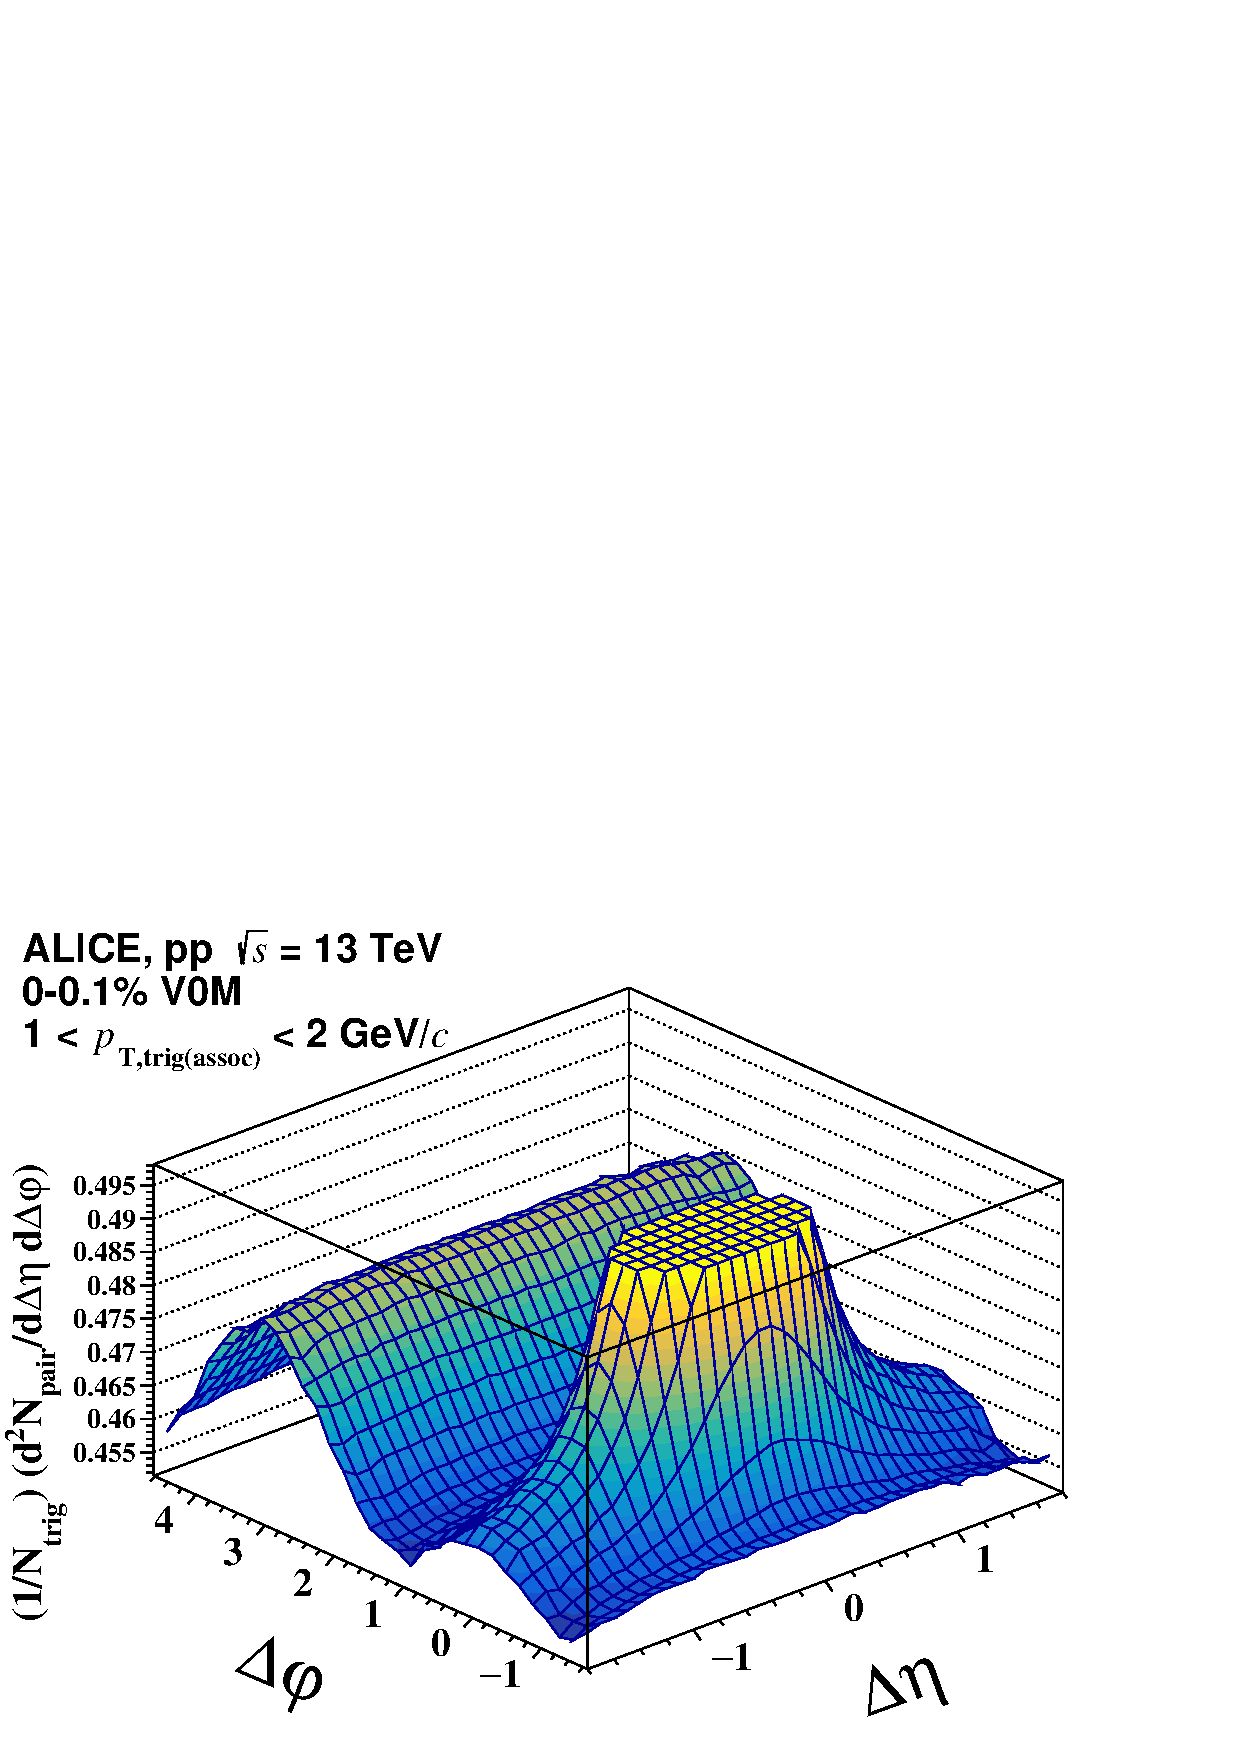
\includegraphics[width=0.31\textwidth]{./figures/corr1.pdf} }
	\subfigure{ \includegraphics[width=0.31\textwidth]{./figures/corr2.pdf} }
	\subfigure{ \includegraphics[width=0.31\textwidth]{./figures/corr3.pdf} }
	\caption{ Two-dimensional associated yield per trigger particle as function of $\Delta\eta$ and $\Delta\varphi$ in 0-0.1\% (left), 5-20\% (middle) and 20-100\% (right) multiplicity class. The interval of transverse momentum of trigger particle and associated particle is 1.0$<\it{p}_{\rm{T}}<$2.0 GeV/\it{c}\rm{}. }

\end{figure}

The one-dimensional $\Delta\varphi$ distribution is shown in Figure 2 for pairs of particles with various $\it{p}_{\rm{T}}$ intervals in very high multiplicity class. The associated yield per trigger particle is compared with CMS results. The near-side peak is highest in the 1.0$<\it{p}_{\rm{T}}<$2.0 interval and gradually decreases with increasing $\it{p}_{\rm{T}}$.

The spectra of the ridge yield is shown in Figure 3 in very high multiplicity class and compared with CMS results. The estimator of particle multiplicity of ALICE is done with forward subsystem(V0), whereas that of CMS is done by mid-rapidity particles meeting with the condition of $|\eta|<$2.4 and $\it{p}_{\rm{T}}>$0.4 GeV/\it{c}\rm{}. Dedicated comparison is conducted and the difference of particle multiplicity is estimated to be about 20\%. Taking into account the difference in acceptance of charged tracks and comparable definition of multiplicity,, the measurements are can be considered comparable with each other.


\begin{figure}
	\centering
	\subfigure{ \includegraphics[width=0.31\textwidth]{./figures/dp1.pdf} }
	\subfigure{ \includegraphics[width=0.31\textwidth]{./figures/dp2.pdf} }
	\subfigure{ \includegraphics[width=0.31\textwidth]{./figures/dp3.pdf} }
	\caption{ One-dimensional $\Delta\varphi$ distribution in the large $\Delta\eta$ with various transverse momentum intervals. Interval of transverse momentum of trigger particle and associated particle is 1.0$<\it{p}_{\rm{T}}<$2.0 GeV/\it{c}\rm{} (left), 2.0$<\it{p}_{\rm{T}}<$3.0 GeV/\it{c}\rm{} (middle) and 3.0$<\it{p}_{\rm{T}}<$4.0 GeV/\it{c}\rm{} (right), respectively. }

\end{figure}
 
\begin{figure}
	\centering
	\subfigure{ \includegraphics[width=0.7\textwidth]{./figures/y.pdf} }
	\caption{(color online) The spectra of ridge yield as function of transverse momentum. The spectrum is compared with CMS result \cite{ridge_pp_1}.}
\end{figure}


\begin{figure}
	\centering
	\subfigure{ \includegraphics[width=0.4\textwidth]{./figures/corrl1.pdf} }
	\subfigure{ \includegraphics[width=0.4\textwidth]{./figures/corrl2.pdf} }
	\caption{ Two-dimensional associated yield per trigger particle as function of $\Delta\eta$ and $\Delta\varphi$ in top 0-0.1\% multiplicity class. The interval of transverse momentum of trigger particle and associated particle is 1.0$<\it{p}_{\rm{T}}<$2.0 GeV/\it{c}\rm{} for the plots. Threshold for leading track selection is 5 GeV/\it{c}\rm{} (left) and 7 GeV/\it{c}\rm{} (right), respectively. }
\end{figure}


\begin{figure}
	\centering
	\subfigure{ \includegraphics[width=0.4\textwidth]{./figures/dpy1.pdf} }
	\subfigure{ \includegraphics[width=0.4\textwidth]{./figures/dpy2.pdf} }
	\caption{ One-dimensional $\Delta\varphi$ distribution in the large $\Delta\eta$ with various leading track selection thresholds. Interval of transverse momentum of trigger particle and associated particle is 1.0$<\it{p}_{\rm{T}}<$2.0 GeV/\it{c}\rm{}. Threshold for leading track selection is 5 GeV/\it{c}\rm{} (left) and 7 GeV/\it{c}\rm{} (right) respectively. }
\end{figure}


\begin{figure}
	\centering
	\subfigure{ \includegraphics[width=0.7\textwidth]{./figures/yl.pdf} }
	\caption{ The ridge yield spectrum with respect to the leading trac∂çk selection. The ridge yields are identical within uncertainties.}
\end{figure}

To further understand the behavior of the ridge in events including hard processes, the two-dimensional associated yield per trigger particle is measured with the leading track selection as shown in Figure 4. The ridge is still visible in the events where $\it{p}_{\rm{T}}^{\rm{Lead}}>$7 GeV/c, which means that the ridge co-exists with hard-scattering in pp collisions. 

The one-dimensional $\Delta\varphi$ distribution with the leading track selection is shown in Figure 5. The near-side yield doesn't change with respect to the leading track requirements within the uncertainties, whereas the away-side peak increases as the leading track requirement gets stronger, presumably because of the increase of the recoil jet yield.

The ridge yield is inspected as a function of the leading track selection in Figure 6. As seen in the previous plots, the ridge yield does not depend on the selection, which indicates that the ridge is not affected significantly by the hardness of the events.

\section{Model Comparison}


\section{Conclusions}

Two-particle angular correlations in large $|\Delta\eta|$ has been measured in very high multiplicity events in pp collsions at $\sqrt{\it{s}}=13$ TeV with ALICE. The measured associated yield is found to be consistent with the previous results from CMS experiment. The ridge yield, for the first time, has been observed in events including hard processes. Furthermore, it is found to be independent of the hardness of the events. This observation is important for the study of the origins of the ridge in small collision systems.

%%%%% acknowledgements
\newenvironment{acknowledgement}{\relax}{\relax}
%\begin{acknowledgement}
%\section*{Acknowledgements}
%\input{acknowledgements.tex}    %%%%%%% done by webmaster team
%\end{acknowledgement}

%%%%%%%% Bibliography (In case of using bibtex generate the bbl requested by arXiv)
%\bibliographystyle{utphys}   % Remember we use title in the biblio
%\bibliography{biblio}
%\input {bibliography.tex}

%%%%%%%%% appendix with author list
\newpage
\appendix
%
%\input{}               %%%%%%%%%%% put your appendices here
%





%\section{The ALICE Collaboration}
%\label{app:collab}
%\input{authorlist-preprint.tex}  %%%%%%% done by webmaster team


\clearpage


\begin{thebibliography}{99}

\bibitem{ridge_aa_1}
CMS Collaboration, "Centrality dependence of dihadron correlations and azimuthal anisotropy harmonics in PbPb collisions at  $\sqrt{\it{s_{\rm{NN}}}} = $2.76 TeV",   Eur. Phys J. C72 (2012).
\bibitem{ridge_aa_2}
ALICE Collaboration, "Anisotropic Flow of Charged Particles in Pb-Pb Collisions at $\sqrt{\it{s_{\rm{NN}}}} = $5.02 TeV",  Phys. Rev. Lett. 116, 132302 (2016).
\bibitem{ridge_pp_1}
CMS Collaboration, Measurement of Long-Range Near-Side Two-Particle Angular Correlations in pp Collisions at $\sqrt{\it{s}} = $13 TeV", Phys. Rev. Lett. 116, 172302 (2016).
\bibitem{ridge_pp_2}
CMS Collaboration, "Evidence for collectivity in pp collisions at the LHC", Phys. Lett. B765 (2017) 193.
\bibitem{ridge_pp_3}
ALICE Collaboration, "Investigations of anisotropic flow using multi-particle azimuthal correlations in pp, p-Pb, Xe-Xe, and Pb-Pb collisions at the LHC", arXiv:1903.01790 [nucl-ex].
\bibitem{ridge_pp_4}
PHENIX Collaboration, "Creation of quark–gluon plasma droplets with three distinct geometries", Nature Phys. 15, 214 (2019), Nature Phys. 13, 535.
\bibitem{ridge_theory_1}
H. Mäntysaari, B. Schenke, C. Shen and P. Tribedy, "Imprints of fluctuating proton shapes on flow in proton-lead collisions at the LHC", Phys. Lett. B772 (2017) 681.
\bibitem{ridge_theory_2}
W. Zhao, Y. Zhou, H. Xu, W. Deng, and H. Song, “Hydrodynamic collectivity in proton?proton collisions at 13 TeV,” Phys. Lett. B780 (2018) 495.
\bibitem{ridge_theory_3}
K. Welsh, J. Singer, and U. W. Heinz, “Initial state fluctuations in collisions between light and heavy ions,” Phys. Rev. C94 no. 2, (2016) 024919.
\bibitem{ridge_theory_4}
M. Greif, C. Greiner, B. Schenke, S. Schlichting, and Z. Xu, “Importance of initial and final state effects for azimuthal correlations in p+Pb collisions,” Phys. Rev. D96 no. 9, (2017) 091504.
\bibitem{ALICEdet}
ALICE Collaboration, “The ALICE experiment at the CERN LHC,” JINST 3 (2008) S08002.
\bibitem{ITSpaper}
ALICE Collaboration, "Performance of the present ALICE Inner Tracking System and studies for the upgrade",  Journal of Instrumentation, 7, June (2012) C06007.
\bibitem{VZEROpaper}
ALICE Collaboration, "Performance of the ALICE VZERO system", JINST 8 (2013) P10016.
\bibitem{TPCpaper}
ALICE Collaboration, "Performance of the ALICE Time Projection Chamber", Physics Procedia 37, (2012) 434.


\end{thebibliography}




\end{document}
